\section{Foundational work} \label{sec:foundations}

%% \begin{figure}
%% \centering
%% \includegraphics[width=.85\textwidth]{poetic-couplets}
%% \caption{A simple flow chart defined in the {\sf FloWr} system \label{fig:simple-flow-chart}}
%% \end{figure}

% AJ *** How is this content relevant? Seems like quite a jump from the last section. I've added a sentence to start the paragraph off ***
In moving towards computational models of serendipity, we are
supported by prior foundational work providing a theoretical framework
and a virtual environment for exploring computational creativity.  In
\citeA{colton-assessingprogress}, we introduced a diagrammatic
formalism for keeping track of progress made in creative computational
systems. An example, pictured in Figure \ref{fig:poetry-progress},
shows how the second iteration of a poetry system gains the ability to
automatically apply aesthetic judgements in order to select a
preferred poem from a larger set of generated examples, once the
programmer has translated (by hand) the relevant aesthetic measures.
\begin{wrapfigure}{l}{4.1cm}
\centering
%\vspace{-30pt}
\resizebox{.23\textwidth}{!}{%
\begin{tikzpicture}[
single/.style={draw, anchor=text, rectangle},
double/.style={draw, anchor=text, rectangle split,rectangle split parts=2},
triple/.style={draw, anchor=text, rectangle split,rectangle split parts=3},
quadruple/.style={draw, anchor=text, rectangle split,rectangle split parts=4}
]
%% beginning of FIRST box
\node[single,scale=0.3] (first) at (0, 0) {
  \tikz{
%\draw[step=1cm,gray,very thin] (-4,-4) grid (4,4);
\node[double] (firstA) at (-2,0) {$<\overline{C_g}>$
  \nodepart{second}{$<E_g>^{*}$}
};
\node[double,right=6mm of firstA.east] (firstB) {$<\overline{A_g}>$
  \nodepart{second}{$[\overline{S}(\overline{a_g}(e_g))]$}
};
\draw [-latex] (firstA.two east) -- (firstB.two west);
\node[above = .01cm of firstB,label={[label distance=2mm]10:{\textbf{P1}}},inner sep=1pt]{};
}
};
%% end of first box

%% beginning of SECOND box
\node[single,scale=0.3,below=3mm of first, inner sep=1mm] (second) {
  \tikz{
%\draw[step=1cm,gray,very thin] (-4,-4) grid (4,4);
\node[double] (firstA) at (-2,0) {$<\overline{C_g}>$
  \nodepart{second}{$<E_g>^{*}$}
};
\node[triple,right=6mm of firstA.one east,yshift=.3mm] (firstB) {$<\overline{A_g}>$
  \nodepart{second}{$\overline{T}(\overline{a_g})$}
  \nodepart{third}{$[S(\overline{a_g}(e_g))]$}
};
\draw [-latex] (firstA.two east) -- (firstB.three west);
\node[above = .01cm of firstB,label={[label distance=2mm]10:{\textbf{P2}}},inner sep=1pt]{};
}
};;
%% end of second box

\draw[->] (first) -- (second);
\end{tikzpicture}}
\vspace{-5pt}
\caption{Progress in developing a poetry system\label{fig:poetry-progress}}
\vspace{-20pt}

\end{wrapfigure}
Progress amounts to more sophisticated processing, and, in the
notation, frequently corresponds to the removal of ``bars'' --
indicating that the system can do something that was formerly done by
a programmer.
%
Thus, this formalism keeps track both of the overall structure of
computational systems, and which actors that are responsible for which
actions within a given instance of the system.
%
As we develop models and systems that people would describe as
serendipitous with reference to the criteria listed in Section
\ref{sec:characteristics}, there will be more to account for.  

\smallskip

For example, we will need to model dynamically changing environments
and a computational version of a prepared mind.
%
To explore these features, are working with a system called {\sf
  FloWr}, portrayed with a screenshot in Figure \ref{fig:being-blunt}.
In {\sf FloWr}, users can construct complex flowcharts composed of
individual ProcessNodes, through which information flows and is
transformed.  The figure depicts a flowchart that has constructed a
poem based on live output from Twitter for the query ``blunt''.  The
dynamic aspects of this environment are threefold: (\emph{i}) some of
the nodes in the flowcharts access online news and social media sites,
which change rapidly from minute to minute; (\emph{ii}) the software
itself can construct new flowcharts, as described in
\cite{charnley2014flowr}; and (\emph{iii}) we are building a community
of ProcessNode builders around the online version of {\sf FloWr},
newly developed since the publication of \cite{charnley2014flowr} in
order to facilitate the direct involvement of other Computational
Creativity researchers.

\begin{figure}
\centering
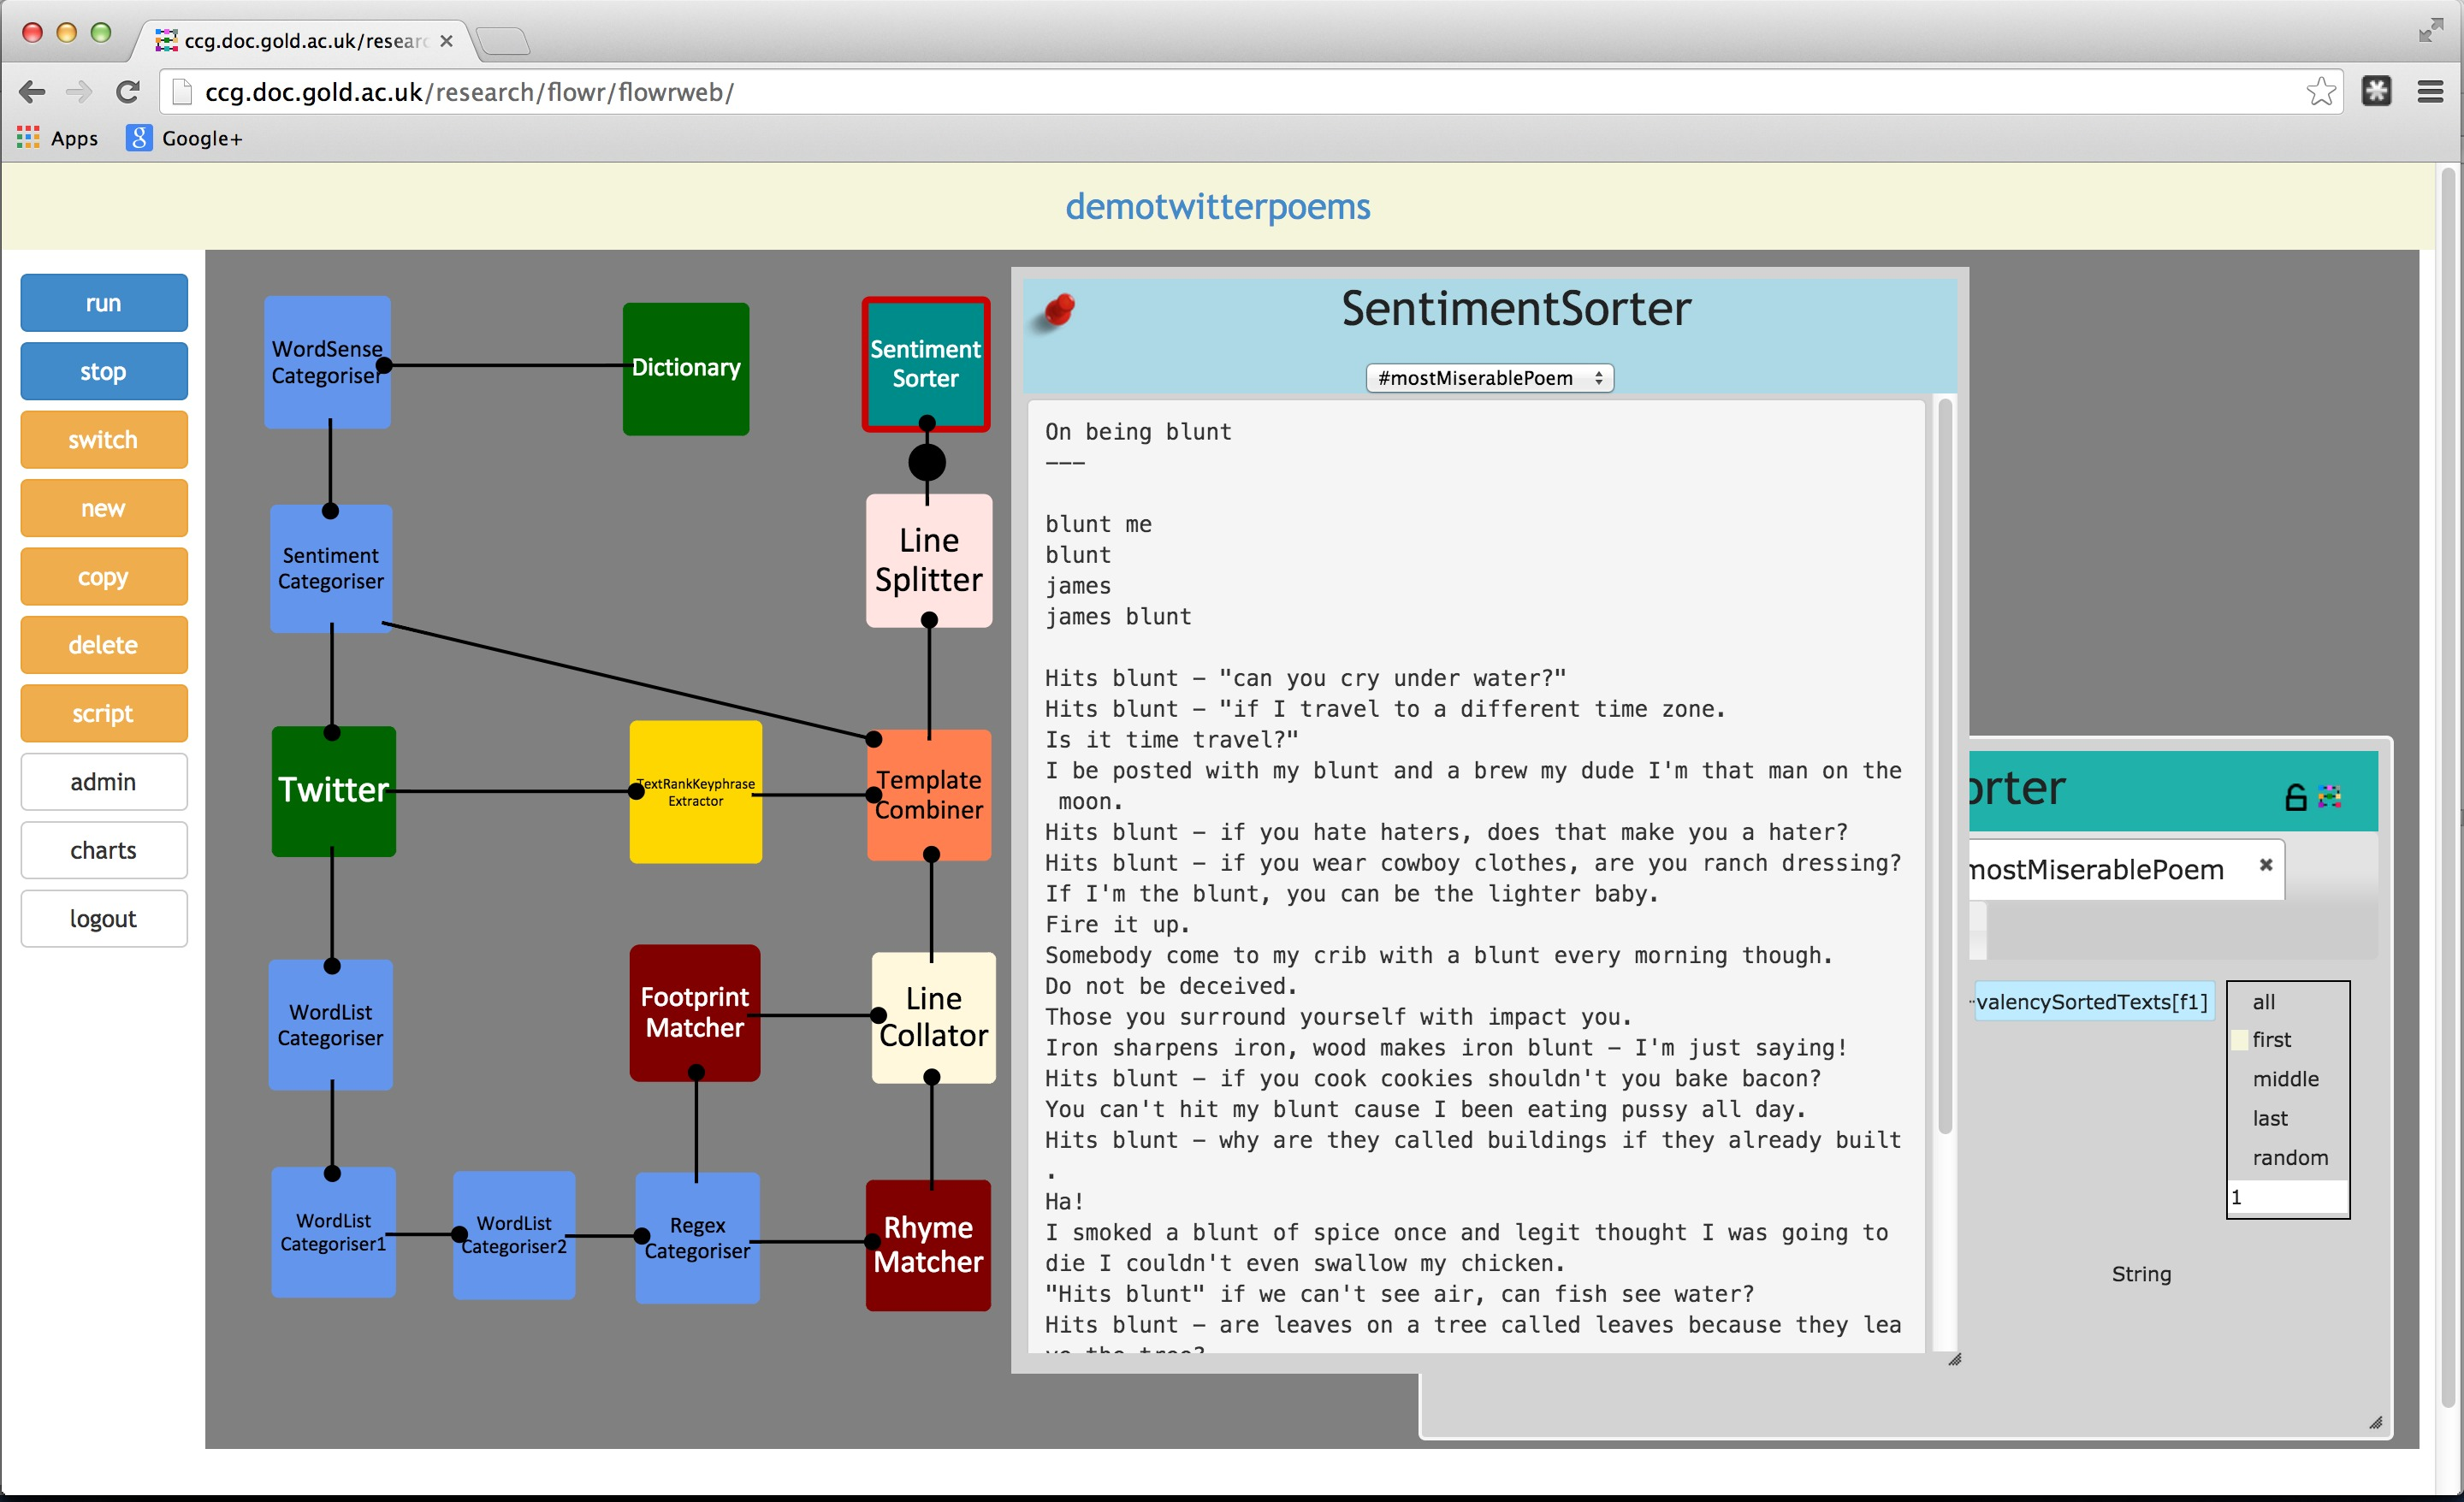
\includegraphics[width=.95\textwidth]{being-blunt}
\caption{A sample poem generated by {\sf FloWr}\label{fig:being-blunt}}
\end{figure}


When {\sf FloWr} constructs flowcharts for itself, while each is
semantically plausible (i.e., they pass the right type of data from
ProcessNode to ProcessNode), many fail -- for instance, because the
available data is limited, or is narrowed down too quickly.  In fact,
the best results in \cite{charnley2014flowr} were at 20\%, i.e., 80\%
of the flowcharts that were constructed failed to produce output.
Each of these failures can be saved as an outstanding problem in {\sf
  FloWr}'s prepared mind.  As data changes and as new nodes are
written and uploaded to the system, {\sf FloWr} will be able to replace nodes,
update data sources, and in general rearrange flowcharts in order to
see if it can fix a broken flowchart.

For instance, suppose a ProcessNode developer wrote and uploaded a
node to mine data from a new social network, in order, say, to produce
textual summaries of world events.  {\sf FloWr} may take that node
and substitute it in the place of an old ``FaceBook'' node in a broken
poetry flowchart. If the replacement worked, and output was produced,
this could be seen as a serendipitous occurrence: {\sf FloWr} will
have taken advantage of the dynamically changing environment -- in
which new social networks come and go, and in which text summaries may
work better in some cases than in others -- to resolve an outstanding
problem in text generation.

The next stage for the {\sf FloWr} system will be to modify it along
these lines, to make it able to adapt to the dynamically changing
environment, and to perform experiments where we monitor potentially
serendipitous scenarios. Such experiments will be similar to those we
tried with the HR2 system in \cite{pease2013discussion}, but improved
because in this earlier effort, we had to break working processes in
order to serendipitously fix them.  The new experiments, the scenarios
will be more realistic, i.e., there will be a catalogue of genuine
open problems waiting to be solved.  Understanding how to work with
this catalogue and the associated experimental process will, of
course, be used to further the computational model of serendipity.  We
discuss one direction for such experiments in Section
\ref{sec:writers-workshop}.
